\textit{PEASS}\cite{peas} (figura \ref{fig:peass-logo}) son las siglas de \textit{Privilege Escalation Awesome Scripts}. \textit{PEASS} es un conjunto de herramientas utilizadas para la escalada de privilegios en los sistemas \textit{Windows}, \textit{Linux/Unix} y \textit{Mac OS}. Estas herramientas buscan por posibles caminos para la escalada de privilegios local que se puedan explotar. El resultado los imprime con diversos colores para que se puedan visualizar de manera sencilla las distintas fallas de configuración.\\

\begin{figure}[h]
    \centering
    
\includegraphics[width=0.35\textwidth]{images/sections/tools/peass.png}
    \caption{Logo de \textit{PEASS-ng}}
    \label{fig:peass-logo}
\end{figure}

Se denomina \textit{\textbf{WinPEAS}}\footnote{\href{https://github.com/carlospolop/PEASS-ng/tree/master/winPEAS}{Web de \textit{WinPEAS}}} a las herramientas utilizadas para la escalada de privilegios en sistemas \textit{Windows}. Los scripts para \textit{Windows} se pueden encontrar en formato \texttt{.exe} y \texttt{.bat}.\\

\textit{\textbf{LinPEAS}}\footnote{\href{https://github.com/carlospolop/PEASS-ng/tree/master/linPEAS}{Web de \textit{LinPEAS}}} es el script utilizado para la escalada de privilegios en sistemas \textit{Linux/Unix} y \textit{Mac OS} (automáticamente el script detecta si es un sistema \textit{Mac}). Como se puede ver en la siguiente figura (figura \ref{fig:linpeas-help}), \textit{linPEAS} tiene diversas opciones para su uso.

\begin{figure}[h]
    \centering
    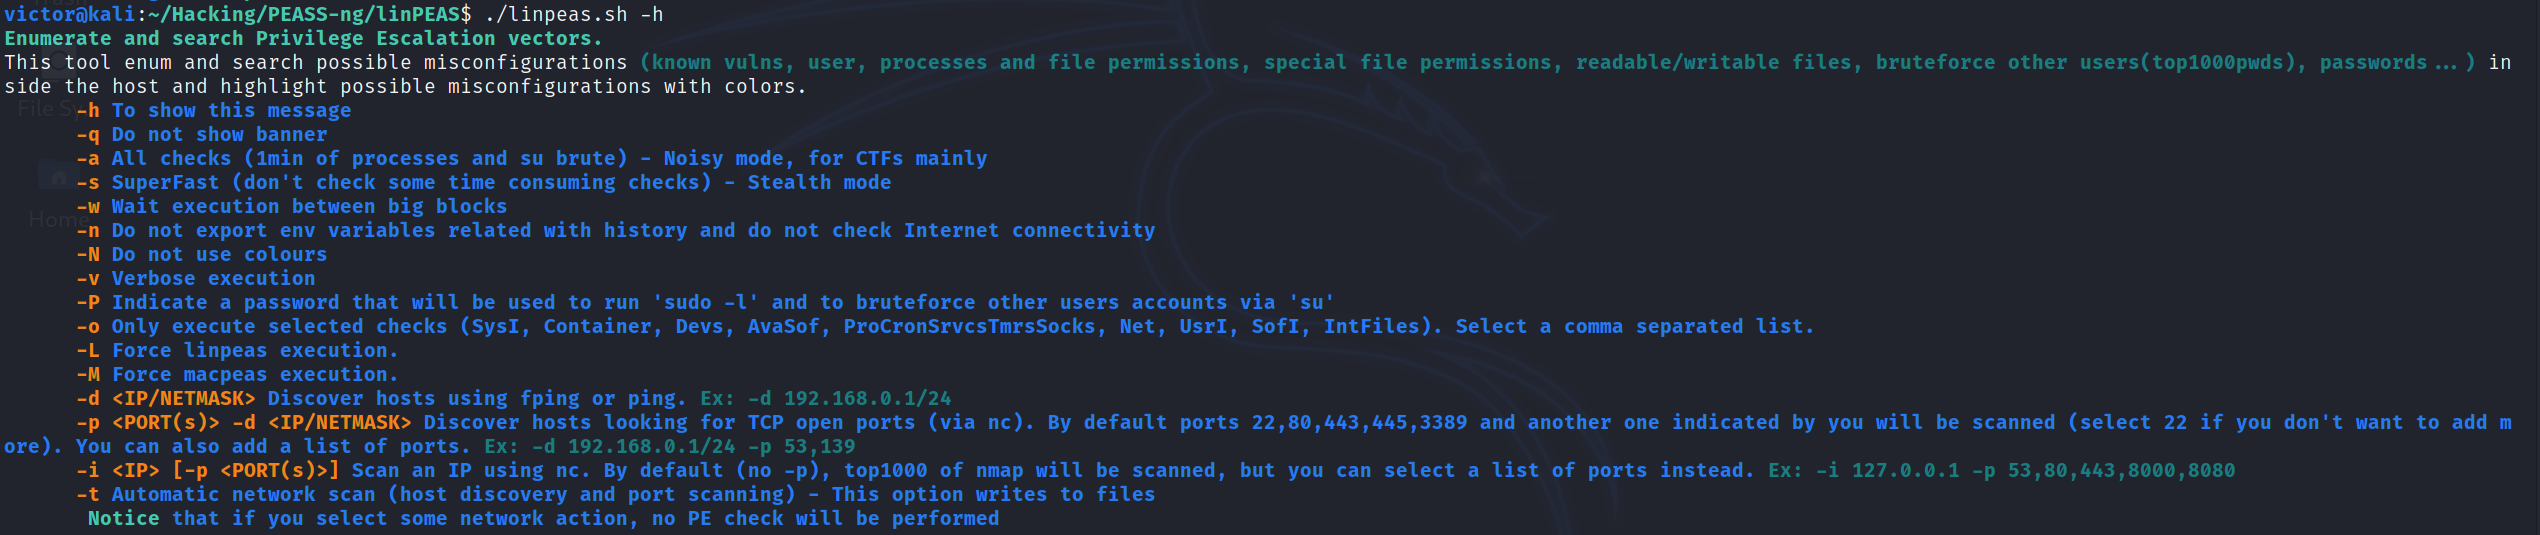
\includegraphics[width=1.0\textwidth]{images/sections/tools/linpeas-help.png}
    \caption{Ayuda \textit{linPEAS}}
    \label{fig:linpeas-help}
\end{figure}

A continuación se muestra un extracto de la salida del script (figura \ref{fig:linpeas-out}).

\begin{figure}[h]
    \centering
    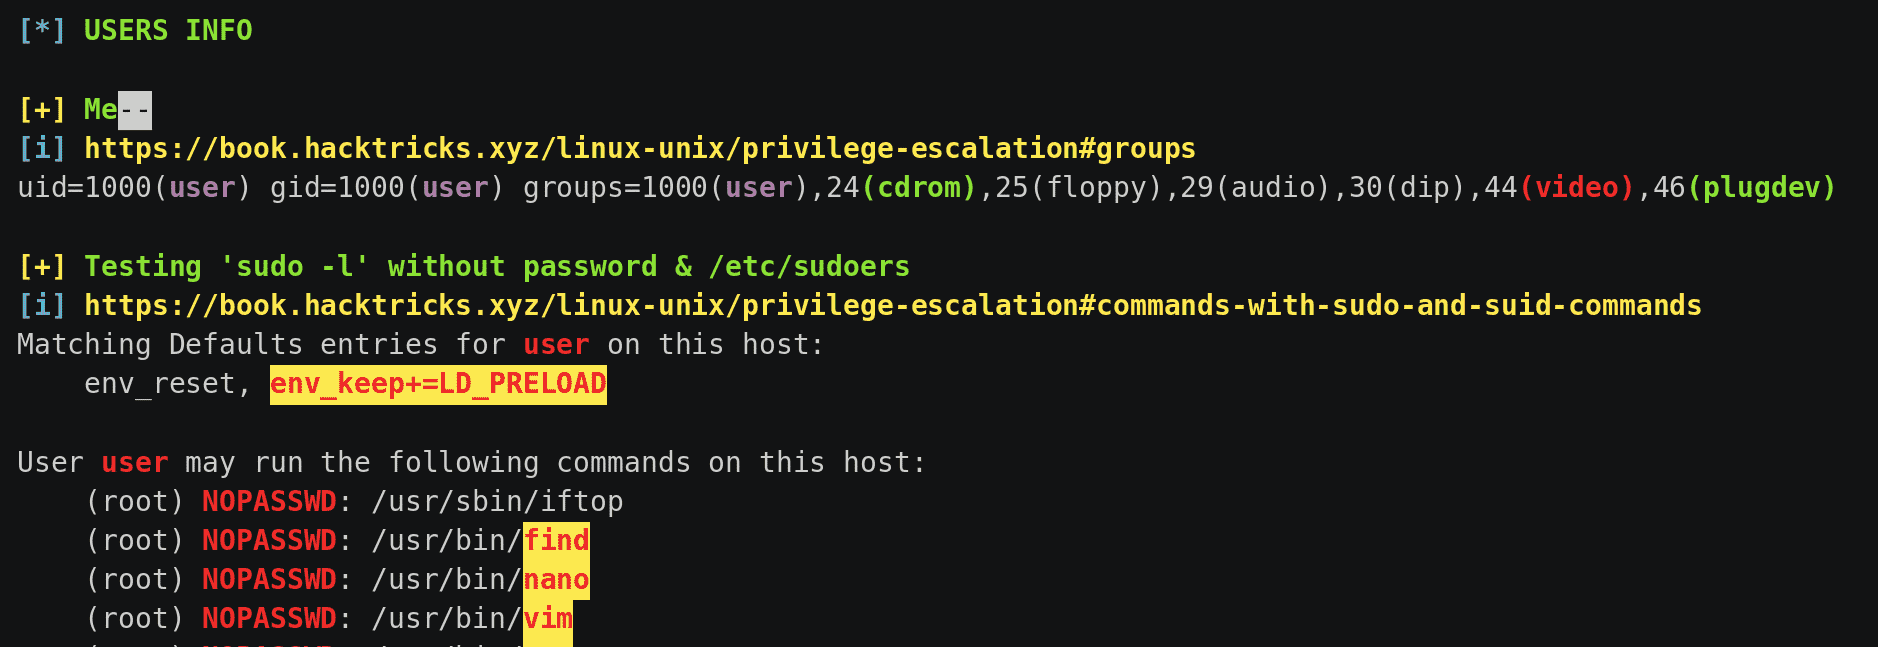
\includegraphics[width=0.8\textwidth]{images/sections/tools/linpeas-out.png}
    \caption{Extracto de la salida de \textit{linPEAS}}
    \label{fig:linpeas-out}
\end{figure}